\documentclass{article}

\renewcommand*\familydefault{\sfdefault}

\usepackage[T1]{fontenc}
\usepackage[utf8x]{inputenc}
\usepackage[left=3cm,right=2cm,top=3cm,bottom=2cm]{geometry} % Márgenes
\usepackage{imakeidx} % Creación de índices
\usepackage{titling} % No tengo claro para qué es esto
\usepackage{fancyhdr} % Cabeceras de página
\usepackage{lastpage} % Módulo para añadir una referencia a la última página
\usepackage[spanish,es-noquoting,es-noshorthands]{babel} % Cadenas de LaTeX traducidas al español 
\usepackage{amsthm} % Paquete de matemáticas
\usepackage{framed} % Marcos 
\usepackage{mdframed} % Más marcos
\usepackage{exmath} % Nuestro querido paquete de utilidades
\usepackage{hyperref} % Para que salgan enlaces en la tabla de contenidos y el glosario
\usepackage{wrapfig} % Figuras flotantes
\usepackage{MathUnicode} % Paquete para poder poner caracteres griegos y demás cosas raras.
\usepackage{listings} % Para poner código.
\usepackage{tikz}

\fancyhf{}
\PrerenderUnicode{ÁáÉéÍíÓóÚúÑñ} % Para que salgan las tildes y demás mierdas en el título.
\fancypagestyle{plain}{%
\lhead{} 
\rhead{} 
\cfoot{\thepage\ de \pageref{LastPage}}
}

% Números en las subsecciones
\setcounter{secnumdepth}{3}

% Ajustes para los enlaces
\hypersetup{
	hyperindex,
    colorlinks,
    citecolor=black,
    filecolor=black,
    linkcolor=black,
    urlcolor=black
}

%%%%% Listings UTF8 %%%%%
\lstset{literate=%
{á}{{\'a}}1
{é}{{\'e}}1
{í}{{\'i}}1
{ó}{{\'o}}1
{ú}{{\'u}}1
{Á}{{\'A}}1
{É}{{\'E}}1
{Í}{{\'I}}1
{É}{{\'O}}1
{Ú}{{\'U}}1
}

\title{Práctica 1 Redes II - Grupo 2301 Pareja 11}
\author{Guillermo Julián Moreno y Víctor de Juan Sanz}
\date{\today}

\begin{document}
\maketitle

\begin{abstract}
En esta práctica se ha implementado con éxito un servidor IRC, siguiendo las especificaciones de los RFC 1459 y 2813, en lenguaje C. Hemos ido algo más allá de programar simplemente un ejercicio para entregar y hemos tratado de crear un sistema robusto, modular, con pruebas exhaustivas, con código limpio y fácil de mantener.

En este documento describimos a grandes rasgos la arquitectura e implementación del servidor. La documentación más exhaustiva a nivel de código se encuentra en los correspondientes ficheros de documentación en formato \textit{man}, \textit{\LaTeX} o \textit{html} generados por Doxygen.
\end{abstract}

\section{Arquitectura}

\subsection{Hilos}

\begin{figure}[hbtp]
\centering
\begin{tikzpicture}
\node[rectangle, draw, inner sep=10pt] (L) at (1,4) {Listener};
\node[rectangle, draw, inner sep=10pt] (R) at (0,0) {Receiver};
\node[rectangle, draw, inner sep=10pt] (P) at (3.5,-2.5) {Processor};
\node[rectangle, draw, inner sep=10pt] (S) at (6,0) {Sender};

\node[circle, draw, inner sep=7pt] (C) at (6,4) {Cliente};

\draw[->] (C) -- node[midway,above, sloped] {Establecimiento} node[midway,below, sloped]{conexión} (L);
\draw[->] (L) -- node[midway,above, sloped] {Notificación} node[midway,below, sloped]{nueva conexión} (R);
\draw[->] (C) -- node[midway,above,sloped] {Mensajes S <- C} (R);
\draw[->] (R) -- node[midway,above,sloped] {Mensajes} node[midway,below, sloped]{recibidos} (P);
\draw[->] (P) -- node[midway,above,sloped] {Mensajes} node[midway,below, sloped]{a enviar} (S);
\draw[->] (S) -- node[midway,right] {Mensajes S -> C} (C);
\end{tikzpicture}
\caption{Arquitectura de hilos del servidor.}
\label{imgHilos}
\end{figure}

Nuestro servidor funciona con 4 hilos distribuidos de la siguiente forma (figura \ref{imgHilos}):
\begin{itemize}
\item  Un hilo a la escucha de nuevas conexiones. (\emph{listener})
\item Un hilo que recibe los datos de esas conexiones (\emph{receiver}) y encola los mensajes recibidos mediante una cola de sistema con la que se comunica con el procesador. \textit{receiver} recibe a través de un socket local UNIX las nuevas conexiones que establezca \textit{listener}.
\item El hilo principal o \textit{processor}, que gestiona las estructuras de datos y realiza los cambios necesarios a partir de los comandos. Es el encargado de analizar los mensajes. Los mensajes generados como respuesta se encolarán hacia \textit{sender}.
\item El hilo que envía los mensajes (\emph{sender}). Recibe los mensajes encolados para enviarlos a través del socket correspondiente.
\end{itemize}

El hilo de procesado, \textit{processor}, usa colas XSI (\texttt{msgget}) para recibir los mensajes de \textit{receiver} y enviarlos a \textit{sender}. Para ello se utiliza la estructura \texttt{sockcomm\_data}, que contiene los datos necesarios para procesar el mensaje (socket de origen/destino, mensaje y su longitud). Esta estructura está encapsulada en otra, \texttt{msg\_sockcommdata}, para enviar los datos a través de las colas.

\paragraph{Justificación del diseño}

Encontramos esta arquitectura varias ventajas frente a otras posibilidades, como pueda ser crear hilo por cliente. La principal ventaja que esta arquitectura presenta es que \textbf{no hay problemas de sincronización} entre hilos que acceden a información, que siempre es un problema difícil de resolver. En nuestro caso, sólo hay un único hilo que accede a la información de IRC. Todos los hilos son totalmente independientes entre sí y no comparten datos.

La desventaja de este enfoque es que perdemos fiabilidad. Si un hilo se queda parado, todo el servidor deja de funcionar. Para evitar esto, todas las operaciones con sockets son no bloqueantes, de tal forma que ningún hilo se quedará esperando al enviar o recibir un mensaje, por ejemplo.

\subsection{Estructuras de datos}

En la estructura de datos globales de irc (\texttt{irc\_globdata}) tenemos 2 diccionarios de \textbf{usuarios}. Unos cuya clave es el descriptor del socket de comunicación y otro cuya clave es el nick, pero ambos tienen como valor el puntero a la misma dirección de memoria. La razón de mantener dos estructuras apuntando a los mismos datos es puramente de velocidad. Los usuarios se buscan o bien por el socket de origen (cada usuario se asocia de forma única a una conexión) o bien por su nombre, y sólo la estructura de diccionario (o tabla \textit{hash}) nos permite hacer búsquedas $O(1)$ en ambos casos.

Con los \textbf{canales} tenemos algo muy parecido: un diccionario (por la velocidad de acceso) y una lista (para poder iterar).

La implementación de esta librería de diccionario y de lista (ambos de punteros a void) fueron implementadas por nosotros en la asignatura Proyecto de Programación y han sido reutilizadas. 

El resto de estructuras de datos de IRC están en el archivo \texttt{types.h} y correctamente documentadas en el manual (carpetas \texttt{man}, \texttt{html} y \texttt{latex/refman.pdf}).

\subsection{Código}

Pasamos ahora a describir la estructura de nuestro código y los archivos más destacados

\begin{itemize}
\item \texttt{includes} Contiene todos los archivos \texttt{.h}.
\begin{itemize}
\item \texttt{types.h} Archivo con todos los tipos y estructuras fundamentales del servidor.
\item \texttt{errors.h} Códigos de error para la interpretación del valor de retorno de nuestras funciones.
\end{itemize}
\item \texttt{src} Contiene los archivos de código principales, incluyendo \texttt{main} y las funciones específicas de IRC.
\begin{itemize}
\item \texttt{irc\_funs.c} Implementaciones de cada uno de los comandos de IRC.
\item \texttt{irc\_core.c} Funciones de manejo de las estructuras de datos del servidor IRC.
\item \texttt{irc\_processor.c} Funciones auxiliares de manejo y procesado de mensajes IRC.
\end{itemize}
\item \texttt{srclib} Contiene las distintas librerías que usamos en el programa.

\begin{itemize}
\item \texttt{libcollections} Contiene \texttt{list} y \texttt{dictionary}, las dos colecciones que usamos en la práctica.
\item \texttt{libcommander} Contiene un intérprete de comandos general junto con un hilo de procesado.
\item \texttt{libjsmn} Una \href{http://zserge.bitbucket.org/jsmn.html}{librería de terceros} que incluye un analizador simple de JSON en pocas líneas de código y sin dependencias extra.
\item \texttt{libsockets} Todas las funciones necesarias para el manejo de socket, incluyendo los hilos de escucha, envío y recepción.
\item \texttt{libstrings} Funciones auxiliares relativas al manejo de cadenas.
\item \texttt{libsysutils} Utilidades del sistema.
\end{itemize}
\item \texttt{tests} Funciones de prueba.
\item \texttt{tools} Scripts y herramientas auxiliares.
\end{itemize}

\section{Pruebas}
Hemos ido realizando test de las funciones que íbamos implementando y los hemos organizado en 3 niveles. 

\begin{itemize}
\item[1] \textbf{Test} Genera el ejecutable llamando a las \textit{suites}.
\item[2] \textbf{Suites} Colecciones de test para cada uno de los módulos, como los hilos o las funciones de IRC.
\item[3] Cada una de las \textit{suites} tiene las funciones que van probando las funcionalidades del programa.
\end{itemize}

Cada una de las funciones de test tiene una nomenclatura común que hace más sencilla la identificación de fallos: \texttt{t\_[nombre de la función a probar]\_\_[situación que se prueba]\_\_[resultado esperado]}.

Estos test nos han permitido probar todas las funciones a medida que íbamos programando, sin esperar a conectar con \textit{Telnet} o con \textit{Xchat}. También nos ha permitido detectar regresiones, fallos que hemos introducido durante el desarrollo sin darnos cuenta, y corregirlos a tiempo. En total, nuestro servidor cuenta con 118 funciones de prueba.

La función más compleja que se prueba es la de \textit{daemonizar}. Usando varios procesos y semáforos, conseguimos automatizar la prueba: creamos un nuevo proceso que \textit{se daemoniza}. Una vez hecho \textit{daemon}, espera en un semáforo a que el proceso principal verifique que el \textit{daemon} cuelga de init y después se cierra liberando los recursos.

Sin embargo, hemos detectado un problema: el kernel de linux 3.11.0-18 no permite daemonizar como los anteriores. Este es el kernel que utiliza Ubuntu 13.10 (instalado en el ordenador de Víctor) por lo que este test falla en su ordenador. No hemos podido arreglar este problema, y ya lo comentamos en clase. Sin embargo nos hemos asegurado de comprobar que funciona correctamente ejecutándolo en otros sistemas.

Además de todas las pruebas automáticas y con XChat/Telnet, hemos pasado regularmente el analizador estático de \textit{clang} para encontrar ciertos fallos en el código detectables antes de la ejecución, como uso de estructuras sin inicializar o uso después de liberar memoria.

\section{Rendimiento}

Hemos hecho varias pruebas para verificar el rendimiento de nuestro servidor. Para ello hemos usado el script \texttt{crazymonkey.py}, que crea múltiples hilos que se conectan al servidor y que envían comandos predefinidos de forma aleatoria. Hemos creado diferentes perfiles de prueba con varios parámetros de intervalo de envío de comandos, clientes conectados y más.s

La medida del tiempo de respuesta se hace con el comando \textit{PING}. El hilo principal del script envía un comando \textit{PING} y mide el tiempo que tarda hasta recibir el correspondiente \textit{PONG}. No han sido necesarios identificadores ya que en ningún momento el script está esperando respuesta a más de un \textit{PING}.

En cuanto a los hilos auxiliares, escogen un comando aleatorio de una lista predefinida:

\begin{verbatim}
	"NICK {nick}",
	"JOIN {channel}",
	"PART {channel}",
	"PRIVMSG {user} :{message}",
	"PRIVMSG {channel} :{message}"
\end{verbatim}

Esto es, comandos de cambio de nombre, entrada y salida de canales y envío de mensajes a usuarios y canales. Tanto los usuarios como los canales se obtienen de listas fijas, globales para todos los hilos, de tal forma que se simula una actividad más o menos real.

Los resultados de la ejecución del programa de pruebas han sido considerablemente buenos. Nuestro servidor soporta sin problemas centenares de usuarios, y los tiempos de respuesta no se disparan. 

Hemos hecho dos pruebas, ambas en el mismo ordenador (Intel Core 2 Duo, 2.26 GHz, 4 GB RAM). La primera era una prueba con el perfil \textit{crazyconns}, que llega a conectar hasta mil clientes al servidor sin enviar ningún comando. 

En este caso, tal y como se ve en la figura \ref{imgCrazyconns}, la media de tiempo de respuesta es de algo menos de 3 milisegundos, con un crecimiento muy lento. Además, el servidor se recuperó sin ningún problema del cierre de esas mil conexiones de forma simultánea.

\begin{figure}[hbtp]
\centering
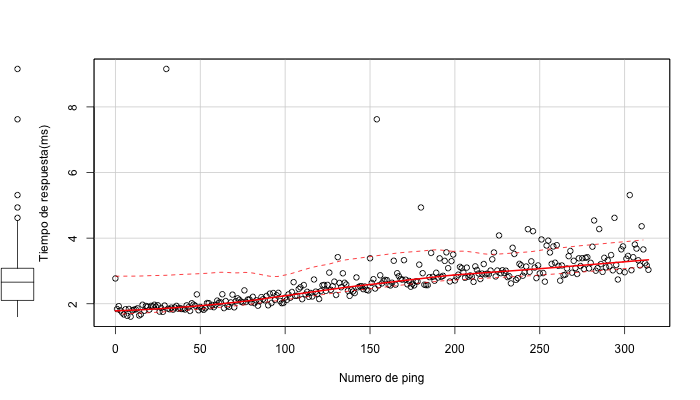
\includegraphics[width=0.8\textwidth]{scatter.png}
\caption{Respuestas con perfil \textit{crazyconns}. El intervalo entre pings es de 200 milisegundos, y aproximadamente cada 15 pings se conectan 50 nuevos clientes.}
\label{imgCrazyconns}
\end{figure}

También queríamos comprobar el rendimiento cuando los usuarios están enviando mensajes. Para ello usamos el perfil \textit{longrun}, obteniendo los resultados de la figura \ref{imgLongrun} con hasta 500 usuarios (no probamos hasta más usuarios porque el script en Python no es muy eficiente y llegaba a parar el ordenador al enviar muchos mensajes).

\begin{figure}[hbtp]
\centering
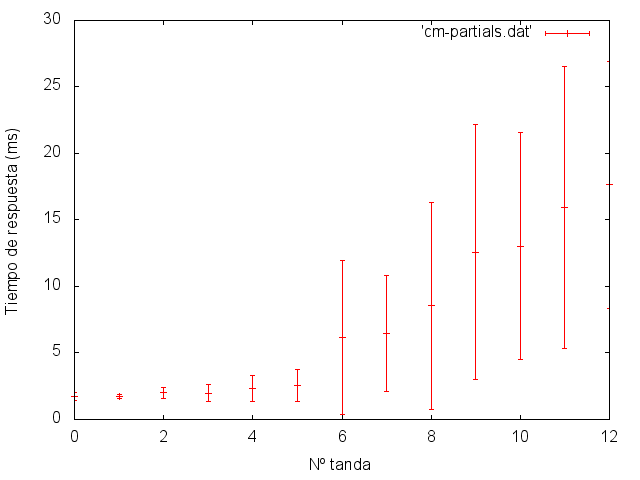
\includegraphics[width=0.8\textwidth]{longrun.png}
\caption{Respuestas con perfil \textit{longrun}. Cada tanda representa cuarenta clientes más conectados, las barras de error indica la desviación típica de los tiempos de respuesta en cada tanda.}
\label{imgLongrun}
\end{figure}

De nuevo, los resultados son buenos, más aún teniendo en cuenta que es un caso más exigente que un escenario real, donde los clientes envían comandos en intervalos más espaciados. Sería conveniente estudiar la razón del aumento de la variabilidad de los tiempos de respuesta al aumentar el número de clientes, aunque en ningún caso se sale de valores razonables.

Además, durante la duración de las pruebas monitorizamos el consumo de CPU y memoria del servidor, que en ningún momento pasó del 20\% ni de 1MB respectivamente. Así mismo, aprovechamos para comprobar con \textit{valgrind} que no había fugas de memoria.



\section{Uso}

El \textit{daemon} se arranca ejecutando el comando \texttt{bin/G-2301-11-P1-main}. Los logs se guardan en en el registro del sistema con el prefijo \textit{redirc}. En caso de querer parar el servidor, el comando \texttt{bin/G-2301-11-P1-main stop} cerrará el servidor ordenadamente.

El servidor lee parámetros de configuración del fichero \texttt{redirc.conf}. De momento los parámetros son únicamente la lista de operadores del servidor y sus contraseñas, en formato JSON no estricto.

Para ejecutar los tests, simplemente hay que ejecutar \texttt{bin/G-2301-11-P1-test}, y los resultados saldrán por pantalla. El ejecutable de pruebas tiene comandos adicionales para ejecutar sólo suites específicas (\texttt{include suite1 suite2 ...}) o excluirlas (\texttt{exclude suite1 suite2 ...}).

\subsection{Makefile}

Nuestro Makefile cuenta con varios objetivos que pasamos a comentar:

\begin{description}
\item[debug] Compilación con banderas de depuración (\textit{-DDEBUG -ggdb}) del ejecutable principal.
\item[no-daemon] Compilación con la bandera \texttt{NODAEMON} definida que evita que el servidor se \textit{daemonice}. Especialmente útil a la hora de depurar con \textit{gdb/lldb} o ejecutar con \textit{valgrind}.
\item[clean] Limpieza de ficheros ejecutables, de compilación y documentación autogenerada.
\item[test] Compilación con banderas de depuración del ejecutable de pruebas.
\item[docs] Generación de manuales con \textit{doxygen} y compilación de documentos LaTeX (esta memoria y el manual de referencia de Doxygen). 
\item[docclean] Limpieza de la documentación generada automáticamente.
\item[pack] Renombrado de archivos para cumplir con las especificaciones del enunciado y empaquetado de la práctica.
\end{description}

\section{Conclusiones}

Hemos descubierto la importancia de ir trabajando bien poco a poco y no hacer \textit{apaños}. El empleo de test nos ha facilitado mucho la tarea. 

No solo con los test, sino también la documentación. Al ir documentando correctamente el código luego hemos podido autogenerar el manual con \texttt{doxygen}. Solo tuvimos que completar algunos ficheros que no estaban documentados (como los reciclados de Proyecto de Programación).

Por último, el empleo de herramientas auxiliares para facilitarnos trabajo, especialmente en los tests. Por ejemplo, \texttt{crazymonkey} para comprobar el rendimiento o una herramienta de la que disponemos para generar e ir añadiendo a \texttt{test.c} y a las suites los test que nos interesaban, de tal forma que sólo hacía falta rellenar el código del test, 

Desde el punto de vista técnico, la arquitectura de hilos que hemos implementado no ha dado problemas y ha hecho realmente fácil el desarrollo al no tener que preocuparnos de semáforos ni sincronización. También hemos visto la importancia de crear funciones cortas (aunque en algún caso, como en ciertas funciones IRC en \texttt{irc\_funs.c}, no lo hemos podido cumplir) y reusables, para acelerar todo lo posible el desarrollo y reducir la cantidad de código que escribimos.

\end{document}
